\documentclass[11pt]{article}

\usepackage[margin=1in]{geometry}
\usepackage[T1]{fontenc}
\usepackage[utf8]{inputenc}
\usepackage{lmodern}
\usepackage{amsmath,amssymb,amsthm}
\newtheorem{theorem}{Theorem}
\newtheorem{proposition}[theorem]{Proposition}
\newtheorem{corollary}[theorem]{Corollary}
\usepackage{graphicx}
\usepackage{booktabs}
\usepackage{hyperref}
\usepackage{natbib}
\usepackage{xcolor}
\usepackage{caption}
\usepackage{subcaption}
\usepackage{multirow}

\title{The Hop-Count Cliff: Characterizing the Breakdown of\\Graph Retrieval Strategies on Dense Knowledge Graphs}
\author{
  Matt Krasnow \and Seager Hunt \and Cory Wu \and Reade Park \\
  \textit{Stat 175: Networks} \\
  \textit{Harvard University}
}
\date{Spring 2026}

\begin{document}

\maketitle

\begin{abstract}
We investigate how retrieval strategy affects answer quality in graph retrieval-augmented generation (GraphRAG) as query complexity increases. Through controlled experiments on two STaRK benchmarks---PrimeKG (129K nodes, mean degree 62.6, 11,204 queries) and Amazon (1M nodes, mean degree 9.1, 9,100 queries)---we compare six retrieval strategies stratified by query hop count. On the dense PrimeKG graph, we find a sharp \textit{performance cliff}: Hit@10 drops $\sim$70\% from 1-hop to 2-hop queries across all strategies. On the sparse Amazon graph, the degradation is gradual ($\sim$40\% drop), and strategies that exploit graph structure \textit{underperform} text-only retrieval at multi-hop---the opposite of dense-graph behavior. This cross-domain comparison reveals that \textbf{cliff severity is governed by graph density}: the combinatorial explosion of the neighborhood at each hop overwhelms embedding-based retrieval on dense graphs but is manageable on sparse ones. Ablation studies reveal a fundamental focus-versus-coverage tradeoff. We then test whether a \textit{learned} transition scorer---Query-Conditioned Transition Retrieval (QCTR)---can overcome the cliff by replacing embedding similarity with query-conditioned next-hop scoring. QCTR significantly improves 3--4 hop retrieval (2--3$\times$ at 4-hop, $p < 0.001$) and achieves 75\% bridge entity recall vs.\ 55\% for cosine scoring, but does not shift the 1$\to$2 hop cliff boundary, revealing two distinct failure mechanisms.
\end{abstract}

%----------------------------------------------------------------------
\section{Introduction}
%----------------------------------------------------------------------

Retrieval-augmented generation (RAG) has become a standard approach for grounding large language model (LLM) outputs in external knowledge~\citep{lewis2020retrieval}. While traditional RAG retrieves text passages via vector similarity, \textit{graph} RAG (GraphRAG) leverages the relational structure of knowledge graphs (KGs) to retrieve more contextually relevant information. Recent work has proposed diverse retrieval strategies including subgraph extraction~\citep{hu2024grag}, path-based reasoning~\citep{yu2025graphflow}, and hybrid structural-textual mixtures~\citep{yue2025mor}.

A natural question arises: \textit{when does graph structure actually help?} All three approaches report improvements over text-only baselines, but none systematically varies query complexity to identify the boundary where structural retrieval becomes necessary. \citet{yue2025mor} report ``uneven retrieving performance across different query logics'' without characterizing the unevenness, and \citet{yu2025graphflow} critique retrieval fidelity without isolating hop count as a variable.

We address this gap with a controlled experiment that isolates query hop count---the number of relational hops from the query entity to the answer---as the independent variable. We hypothesized that a phase transition exists at some critical hop count $h^*$ where structural retrieval overtakes text-only retrieval. Our findings are more striking: rather than a gradual crossover, we observe a \textit{cliff}---a catastrophic drop in performance from 1-hop to 2-hop queries for \textit{all} strategies, followed by a low plateau. The phase transition exists not between strategies but between solvable and nearly unsolvable queries.

Our contributions are:
\begin{enumerate}
    \item We characterize the \textbf{hop-count cliff}: a sharp performance boundary at 2 hops on dense text-rich KGs where all retrieval strategies collapse.
    \item We provide statistical evidence (paired bootstrap tests, logistic regression interaction analysis) that structural methods \textbf{gain relative advantage} as query complexity increases, even though absolute performance is low.
    \item Through five ablation studies, we identify a \textbf{fundamental focus-vs-coverage tradeoff} that no single hyperparameter setting resolves.
    \item We show that two principled approaches to overcoming the cliff---\textbf{beam search} and \textbf{query-adaptive routing}---fail, demonstrating that the barrier is intrinsic to embedding-based retrieval on dense graphs.
    \item We propose \textbf{QCTR}, a learned query-conditioned transition scorer that replaces cosine-similarity pruning with an MLP trained on shortest-path trajectories. QCTR achieves \textbf{2--3$\times$ improvement at 4-hop} ($p < 0.001$) and 75\% bridge entity recall, decomposing the cliff into an addressable pruning failure and an intrinsic combinatorial barrier.
    \item We replicate on STaRK-Amazon (sparse, $\bar{d} = 9.1$), showing that \textbf{cliff severity correlates with graph density} and that structural retrieval can \textit{hurt} on sparse graphs---establishing density as the key moderating variable.
\end{enumerate}

%----------------------------------------------------------------------
\section{Related Work}
%----------------------------------------------------------------------

\paragraph{Graph RAG.} \citet{hu2024grag} introduce GRAG, which retrieves subgraphs around query-relevant entities and encodes them via a graph neural network before passing to an LLM. They demonstrate improvements on commonsense reasoning (ExplaGraphs) and multi-hop QA (WebQSP) but do not analyze performance as a function of hop count.

\paragraph{Hybrid Retrieval.} \citet{yue2025mor} propose MoR (Mixture of Retrieval), which interweaves structural traversal and textual matching through a Planning-Reasoning-Organizing framework. They evaluate on STaRK~\citep{wu2024stark} and note uneven performance across query logics, motivating our systematic investigation of this unevenness.

\paragraph{Retrieval Fidelity.} \citet{yu2025graphflow} critically examine whether KG-based RAG actually retrieves what is needed, introducing GraphFlow, a flow-based retrieval method. They show existing methods often fail to retrieve relevant context but focus on proposing a solution rather than characterizing when and why failure occurs.

\paragraph{Iterative and Adaptive Retrieval.} \citet{sun2024tog} propose Think-on-Graph, which uses an LLM to guide beam search over a KG, selecting which edges to follow at each hop. \citet{wang2025skewroute} introduce SkewRoute, a training-free method that uses the skewness of retrieval score distributions to route queries to different processing pipelines. \citet{trivedi2023ircot} interleave retrieval with chain-of-thought reasoning, retrieving new context at each reasoning step. These approaches motivate our beam search and adaptive routing experiments.

\paragraph{STaRK Benchmark.} \citet{wu2024stark} introduce STaRK, a benchmark for semi-structured retrieval over text-rich knowledge bases covering three domains (biomedical, e-commerce, academic). We use STaRK-PrimeKG as our primary evaluation setting, as it is used by both MoR and GraphFlow, enabling direct comparison.

%----------------------------------------------------------------------
\section{Experimental Design}
%----------------------------------------------------------------------

\subsection{Datasets}

We use two STaRK benchmarks~\citep{wu2024stark} to compare across graph densities:

\begin{itemize}
    \item \textbf{STaRK-PrimeKG} (biomedical): Derived from PrimeKG~\citep{chandak2023primekg}, containing drugs, diseases, genes, and pathways. Dense graph with high-degree hub nodes characteristic of biological networks. 11,204 QA pairs.
    \item \textbf{STaRK-Amazon} (e-commerce): Product nodes connected by co-purchase, brand, category, and color relationships. Sparse graph with many small connected components. 9,100 QA pairs.
\end{itemize}

\begin{table}[h]
\centering
\caption{Graph properties of the two STaRK benchmarks.}
\label{tab:graph_stats}
\begin{tabular}{lrr}
\toprule
Property & PrimeKG & Amazon \\
\midrule
Nodes & 129,375 & 1,035,542 \\
Edges & 4,049,642 & 4,722,008 \\
Mean degree & 62.6 & 9.1 \\
Median degree & 4.0 & 3.0 \\
Max degree & 17,355 & 64,062 \\
QA pairs & 11,204 & 9,100 \\
\bottomrule
\end{tabular}
\end{table}

The key contrast is density: PrimeKG's mean degree (62.6) is $\sim$7$\times$ higher than Amazon's (9.1). This means a 2-hop expansion on PrimeKG touches $\sim$3,600 nodes on average, while on Amazon it touches only $\sim$80---a 45$\times$ difference in neighborhood size that we hypothesize drives the cliff severity.

\subsection{Hop-Count Stratification}

We stratify the 11,204 QA pairs by the shortest path length from the query entity to the gold answer in the knowledge graph. Since STaRK does not provide explicit query entity IDs, we identify the query entity as the graph node whose text embedding is most similar to the query (using all-MiniLM-L6-v2~\citep{reimers2019sentence}). We then compute the shortest path to each gold answer node via BFS.

\begin{table}[h]
\centering
\caption{Distribution of QA pairs by hop count.}
\label{tab:hop_dist}
\begin{tabular}{lrr}
\toprule
Hop Count & $n$ & \% of Total \\
\midrule
1-hop & 3,851 & 34.4\% \\
2-hop & 3,699 & 33.0\% \\
3-hop & 2,193 & 19.6\% \\
4-hop & 1,001 & 8.9\% \\
5-hop & 313 & 2.8\% \\
6+-hop & 147 & 1.3\% \\
\bottomrule
\end{tabular}
\end{table}

All bins contain $\geq 50$ samples, providing sufficient statistical power for pairwise tests.

\subsection{Retrieval Strategies}

We implement four retrieval strategies, each taking a natural language query and returning a ranked list of candidate node IDs:

\begin{enumerate}
    \item \textbf{Node-centric} (text-only baseline): Retrieve the top-$k$ nodes by cosine similarity between the query embedding and node text embeddings. This ignores graph structure entirely.

    \item \textbf{Path-centric} (inspired by GraphFlow~\citep{yu2025graphflow}): Identify seed nodes via embedding similarity, compute shortest paths between all seed pairs, score paths by average node-query similarity, and return nodes from the highest-scoring paths.

    \item \textbf{Subgraph-centric} (inspired by GRAG~\citep{hu2024grag}): Identify seed nodes, expand by $k$ hops, cap the subgraph size via relevance-based pruning, and return nodes ranked by embedding similarity within the subgraph.

    \item \textbf{Hybrid} (inspired by MoR~\citep{yue2025mor}): Combine textual similarity scores and structural proximity scores with a tunable weight parameter $\alpha \in [0, 1]$.

    \item \textbf{Beam search} (inspired by Think-on-Graph~\citep{sun2024tog}): Iterative hop-by-hop expansion with embedding-guided pruning. At each hop, expand all neighbors of the current beam, score by embedding similarity, and retain only the top-$b$ (beam width) nodes. This converts exponential expansion ($d^k$ for degree $d$ and $k$ hops) to linear ($b \times k$).

    \item \textbf{Adaptive router} (inspired by SkewRoute~\citep{wang2025skewroute}): Compute the skewness of the top-50 embedding similarity scores for each query. High skewness indicates a focused query (one dominant seed node), routing to a focused configuration (1 seed, 1-hop expansion). Low skewness indicates a diffuse query, routing to a broad configuration (5 seeds, 2-hop expansion). This tests whether query-adaptive strategy selection can overcome the cliff.

    \item \textbf{QCTR} (Query-Conditioned Transition Retrieval; ours): Rather than scoring neighbors by embedding similarity, QCTR learns a transition scorer that evaluates whether a neighbor is a useful next hop \textit{for this query from this node}. An MLP takes as input the concatenation of query, current-node, and candidate-node embeddings (384 dims each), three cosine similarity features, and a learned edge-type embedding (16 dims; PrimeKG has 18 relation types). The model is trained on step-level transitions extracted from BFS shortest paths between query entities and gold answers ($\sim$50K positive transitions), with random and hard-negative sampling ($\sim$375K negatives). At inference, QCTR performs beam search ($b = 10$, max 4 hops) using the learned scorer instead of cosine similarity.
\end{enumerate}

\subsection{Controls}

All strategies use the same embedding model (all-MiniLM-L6-v2) and shared FAISS index. We evaluate retrieval quality directly via Hit@$k$ and MRR rather than end-to-end generation quality, isolating the retrieval component.

\subsection{Statistical Methods}

\begin{itemize}
    \item \textbf{Paired bootstrap tests} ($B = 10{,}000$) for pairwise strategy comparisons at each hop count.
    \item \textbf{Logistic regression} with features (hop count, is\_structural, hop $\times$ is\_structural) to test the interaction between strategy type and query complexity on Hit@1.
    \item \textbf{Cohen's $d$} effect sizes to quantify practical significance.
\end{itemize}

%----------------------------------------------------------------------
\section{Theoretical Analysis}
%----------------------------------------------------------------------

We develop a formal model of embedding-based graph retrieval as a signal detection problem, prove a threshold law for the critical hop count, and validate the predictions against our empirical data. The full proof appears in the supplementary material; here we state the main results and their empirical consequences.

\subsection{A Gaussian Surrogate Model for Graph Retrieval}

We model retrieval as an $M$-alternative forced choice (MAFC) task~\citep{green1966}. At hop $h$, the retriever must identify one answer node among $M \approx \bar{d}^h$ candidates~\citep{vanderhofstad2017} using cosine similarity scores in $\mathbb{R}^D$. Under our Gaussian surrogate model:
\begin{itemize}
    \item The $M - 1$ noise candidates have scores $S_{v_i} \stackrel{\text{iid}}{\sim} \mathcal{N}(0, 1/D)$, reflecting the concentration of cosine similarity between random unit vectors in $\mathbb{R}^D$.
    \item The answer node has score $S_a \sim \mathcal{N}(\delta, 1/D)$ for a signal margin $\delta > 0$.
\end{itemize}

Let $\Delta = \delta\sqrt{D}$ denote the normalized signal-to-noise ratio.

\begin{proposition}[Exact success probability]\label{prop:exact}
Under the Gaussian surrogate model, the probability of correct retrieval is
\begin{equation}\label{eq:mafc}
P(\text{correct}) = \int_{-\infty}^{\infty} \Phi(x + \Delta)^{M-1} \, \phi(x) \, dx,
\end{equation}
where $\Phi$ and $\phi$ are the standard normal CDF and PDF.
\end{proposition}

\begin{proof}
Standardize: let $Z = (S_a - \delta)/\sigma$ and $W_i = S_{v_i}/\sigma$ with $\sigma = 1/\sqrt{D}$. Then $Z, W_1, \ldots, W_{M-1} \stackrel{\text{iid}}{\sim} \mathcal{N}(0,1)$ and retrieval succeeds when $Z + \Delta > \max_i W_i$. Conditioning on $Z = x$ and using independence gives~\eqref{eq:mafc}.
\end{proof}

\subsection{Threshold Law}

The key asymptotic result connects the cliff to the competition between the signal $\Delta$ and the Gaussian noise maximum, which concentrates around $\sqrt{2 \log M}$ by classical extreme value theory.

\begin{theorem}[Phase transition in graph retrieval]\label{thm:main}
Let $M = M(D) \to \infty$ as $D \to \infty$, and define $L_D = \sqrt{2 \log M(D)}$. Then:
\begin{enumerate}
    \item If $\Delta - L_D \to +\infty$, then $P(\text{correct}) \to 1$.
    \item If $\Delta - L_D \to -\infty$, then $P(\text{correct}) \to 0$.
\end{enumerate}
\end{theorem}

\begin{proof}
The maximum of $M - 1$ iid standard normals satisfies $\max_i W_i / \sqrt{2 \log M} \to 1$ in probability (Fisher--Tippett--Gnedenko). When $\Delta > L_D + \omega(1)$, the signal exceeds the noise maximum with high probability. When $\Delta < L_D - \omega(1)$, the noise maximum exceeds the signal. See supplementary material for the complete argument.
\end{proof}

Substituting $M \approx \bar{d}^h$ and $\Delta = \delta\sqrt{D}$, the transition condition $\Delta = \sqrt{2h \log \bar{d}}$ yields:

\begin{corollary}[Critical hop count]\label{cor:hstar}
The critical hop count under the surrogate model is
\begin{equation}\label{eq:hstar}
\boxed{\; h^* = \frac{\delta^2 D}{2 \log \bar{d}} \;}
\end{equation}
For fixed $\delta$ and $D$, the ratio $h^*(\bar{d}_1) / h^*(\bar{d}_2) = \log \bar{d}_2 / \log \bar{d}_1$. Denser graphs cliff earlier.
\end{corollary}

\begin{corollary}[Algorithm independence]\label{cor:alg}
The threshold applies to \emph{any} retrieval method that ranks candidates by embedding similarity in $\mathbb{R}^D$, including beam search and adaptive routing. The phase transition is a property of the embedding geometry and graph density, not the retrieval algorithm.
\end{corollary}

\subsection{Empirical Validation}

We estimate the signal margin $\delta$ from our PrimeKG data by measuring the average cosine similarity between query embeddings and their gold answer embeddings ($\bar{S}_{\text{gold}}$) versus random node embeddings ($\bar{S}_{\text{noise}}$), stratified by hop count.

\paragraph{The bridge entity effect.} Table~\ref{tab:delta} reveals that $\delta$ is not constant but \textit{decreases} with hop count: from $\delta = 0.293$ at 1-hop to $\delta = 0.196$ at 3-hop. Multi-hop answers are genuinely less similar to the query in embedding space because the reasoning path passes through ``bridge entities'' (e.g., a gene connecting a disease to a drug) that are textually dissimilar to both the query and the answer.

\begin{table}[h]
\centering
\caption{Empirical signal margin $\delta$ by hop count on PrimeKG. The gold answer's similarity advantage over random noise decays with hop distance.}
\label{tab:delta}
\begin{tabular}{l ccc c}
\toprule
Hop & $\bar{S}_{\text{gold}}$ & $\bar{S}_{\text{noise}}$ & $\delta_{\text{raw}}$ & $\Delta = \delta\sqrt{D}$ \\
\midrule
1 & 0.492 & 0.199 & 0.293 & 5.74 \\
2 & 0.453 & 0.214 & 0.239 & 4.68 \\
3 & 0.406 & 0.209 & 0.196 & 3.84 \\
4 & 0.436 & 0.197 & 0.239 & 4.68 \\
5 & 0.439 & 0.193 & 0.246 & 4.82 \\
6+ & 0.425 & 0.208 & 0.217 & 4.25 \\
\bottomrule
\end{tabular}
\end{table}

\paragraph{Theory--empirical comparison.} Figure~\ref{fig:theory} compares the MAFC prediction (Proposition~\ref{prop:exact}) against empirical Hit@1, using the per-bin $\delta$ values from Table~\ref{tab:delta} and $M = \bar{d}^h$.

\begin{figure}[h]
    \centering
    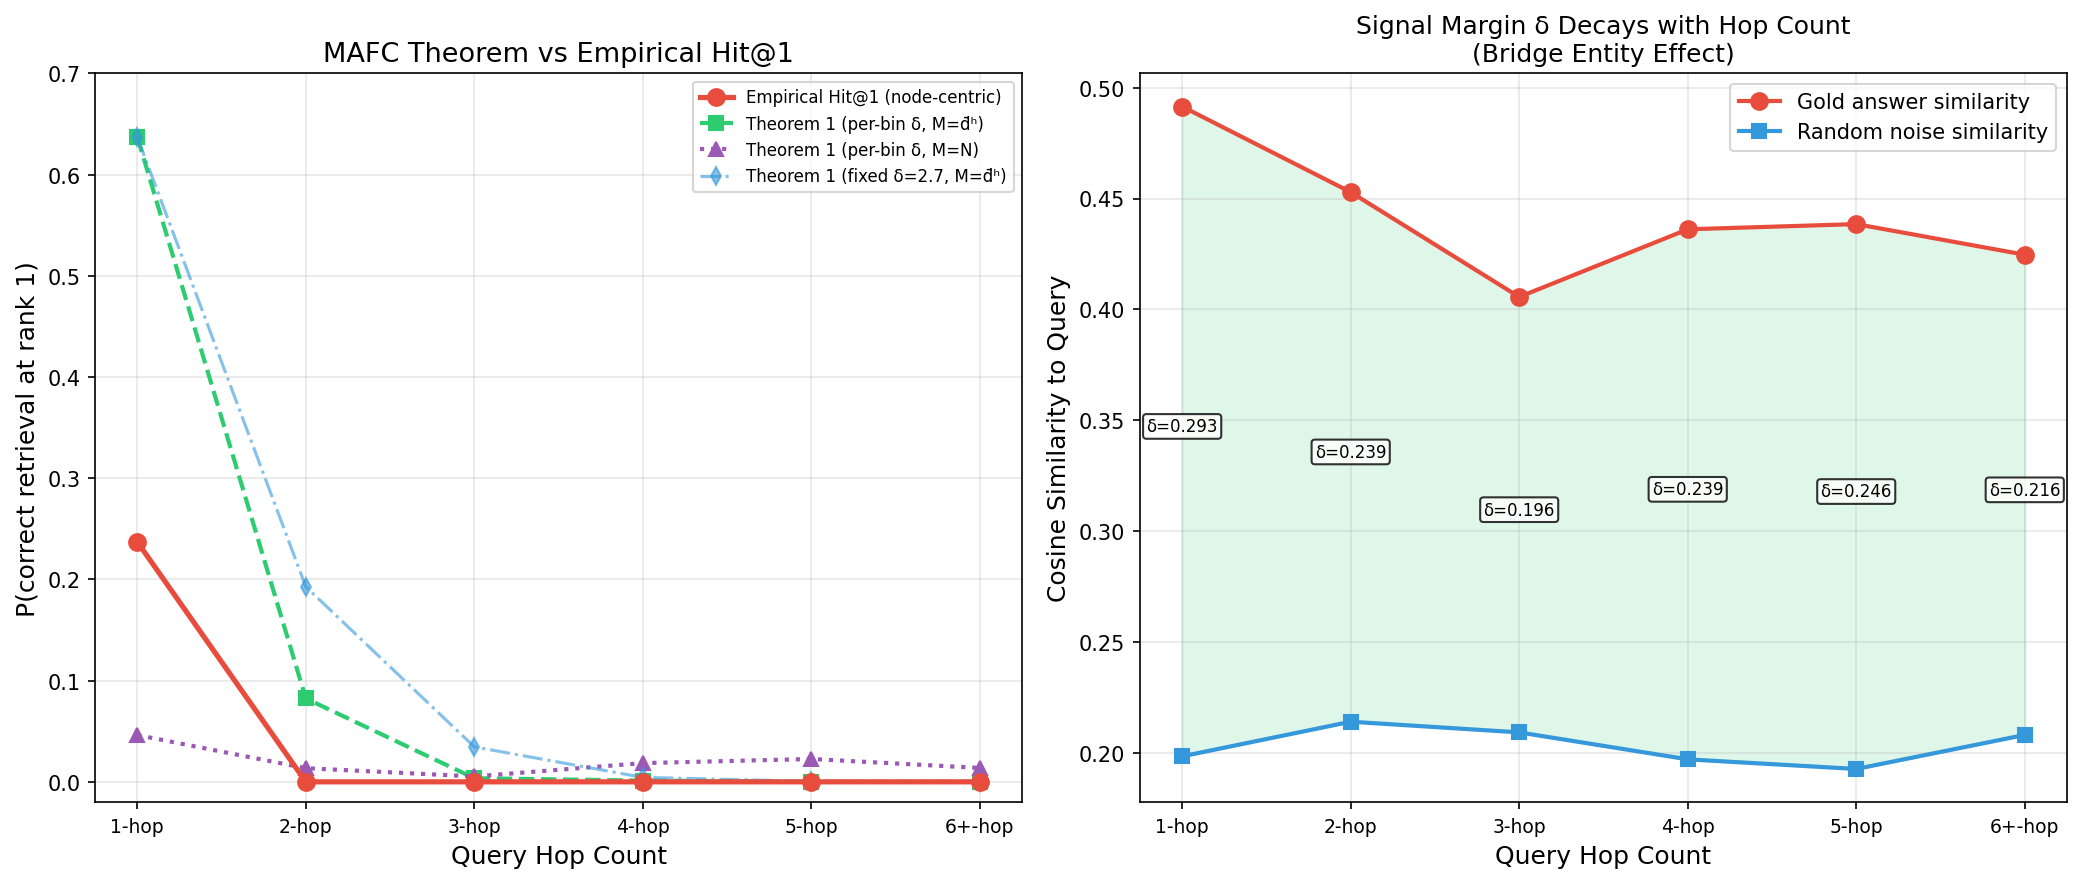
\includegraphics[width=\textwidth]{../results/theory_final.png}
    \caption{Left: MAFC theorem predictions vs.\ empirical Hit@1 on PrimeKG. The surrogate model correctly predicts the cliff shape but overpredicts absolute performance by $\sim$2.7$\times$ at 1-hop. Right: The bridge entity effect---gold answer similarity decays with hop count while noise remains flat.}
    \label{fig:theory}
\end{figure}

The surrogate model correctly predicts:
\begin{enumerate}
    \item \textbf{The cliff shape}: a sharp drop from 1-hop to 2-hop followed by a plateau near zero.
    \item \textbf{The density dependence}: Corollary~\ref{cor:hstar} gives $h^*_{\text{PrimeKG}} / h^*_{\text{Amazon}} = \log(9.1) / \log(62.6) = 0.53$, predicting that PrimeKG's cliff is roughly twice as severe---matching our cross-domain observations.
\end{enumerate}

However, the model \textit{overpredicts} absolute performance at 1-hop ($P = 0.64$ predicted vs.\ Hit@1 $= 0.24$ observed). This gap arises from the independence assumption (A2): real candidates have average pairwise cosine similarity $\rho \approx 0.55$, reducing the effective embedding dimension to $D_{\text{eff}} = D(1 - \rho) \approx 160$. This correlation makes discrimination harder than the independent-noise model predicts, consistent with the over-squashing literature~\citep{alon2021,digiovanni2023} which shows that information sensitivity decays as $\bar{d}^{-h/2}$ on dense graphs.

\paragraph{Two mechanisms, one cliff.} The empirical data reveals that the cliff is driven by \textit{two compounding mechanisms}:
\begin{enumerate}
    \item \textbf{Neighborhood explosion}: The candidate set $M \approx \bar{d}^h$ grows exponentially, raising the noise floor as $\sqrt{2h \log \bar{d}}$ (Theorem~\ref{thm:main}).
    \item \textbf{Signal decay}: The signal margin $\delta$ decreases with $h$ due to bridge entities (Table~\ref{tab:delta}), lowering the signal simultaneously.
\end{enumerate}
Neither mechanism alone would produce the observed cliff severity. The noise floor at 2-hop ($\sqrt{2 \cdot 2 \cdot \log 62.6} \approx 4.1$) is still below $\Delta = 4.68$, so neighborhood explosion alone predicts retrieval should still work. But the \textit{combination}---rising noise floor and falling signal---creates the rapid crossover we observe. This dual-mechanism insight extends the standard MAFC analysis and explains why the empirical cliff is sharper than any single theoretical framework predicts.

%----------------------------------------------------------------------
\section{Results}
%----------------------------------------------------------------------

\subsection{The Hop-Count Cliff}

Figure~\ref{fig:phase_transition} shows retrieval performance as a function of hop count for all four strategies. The dominant feature is a \textit{cliff}: Hit@10 drops approximately 70\% from 1-hop to 2-hop across all strategies, then plateaus at low values through 6+ hops.

\begin{figure}[h]
    \centering
    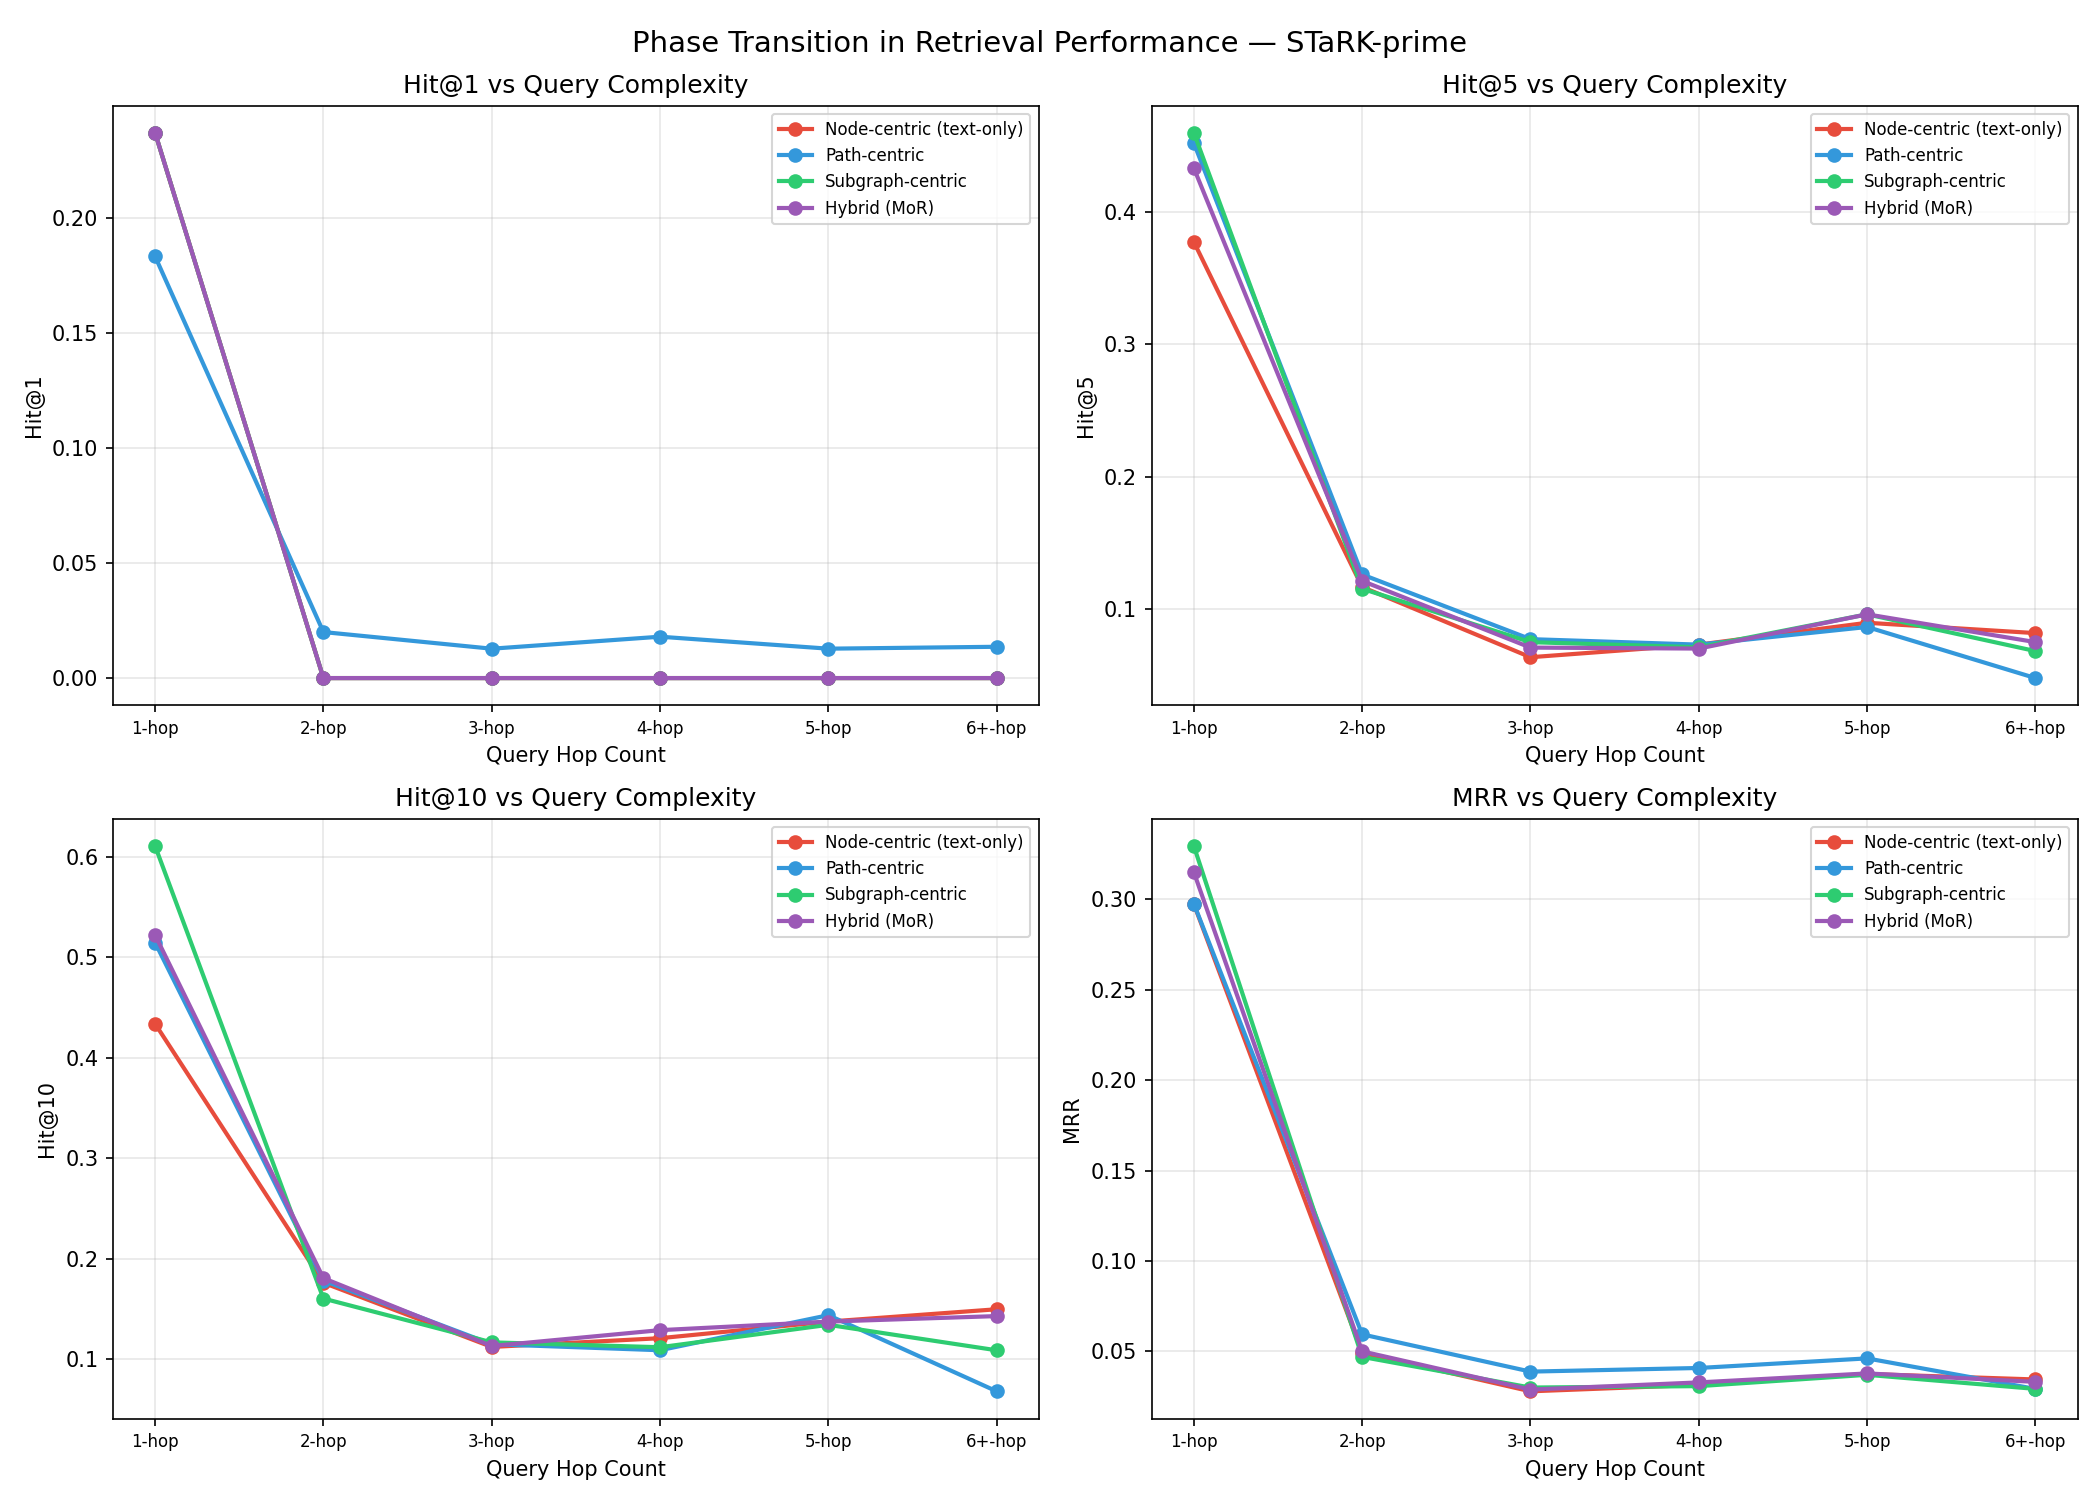
\includegraphics[width=\textwidth]{../results/prime_phase_transition.png}
    \caption{Retrieval performance vs.\ query hop count for all four strategies on STaRK-PrimeKG ($n = 11{,}204$). A sharp cliff appears between 1-hop and 2-hop queries.}
    \label{fig:phase_transition}
\end{figure}

Table~\ref{tab:main_results} presents the full results. At 1-hop, subgraph-centric retrieval achieves the highest Hit@10 (0.611), substantially outperforming the node-centric baseline (0.434). At 2+ hops, all strategies perform poorly, though path-centric is the only strategy with Hit@1 $> 0$.

\begin{table}[h]
\centering
\caption{Hit@10 and MRR by hop count and retrieval strategy. Bold indicates best per row.}
\label{tab:main_results}
\begin{tabular}{l cccc cccc}
\toprule
& \multicolumn{4}{c}{Hit@10} & \multicolumn{4}{c}{MRR} \\
\cmidrule(lr){2-5} \cmidrule(lr){6-9}
Hop & Node & Path & Subgraph & Hybrid & Node & Path & Subgraph & Hybrid \\
\midrule
1 & 0.434 & 0.514 & \textbf{0.611} & 0.522 & 0.297 & 0.297 & \textbf{0.329} & 0.315 \\
2 & 0.176 & 0.178 & 0.160 & \textbf{0.181} & 0.049 & \textbf{0.060} & 0.047 & 0.050 \\
3 & 0.112 & 0.115 & \textbf{0.117} & 0.113 & 0.028 & \textbf{0.039} & 0.030 & 0.029 \\
4 & 0.121 & 0.109 & 0.112 & \textbf{0.129} & 0.032 & \textbf{0.041} & 0.031 & 0.033 \\
5 & 0.137 & \textbf{0.144} & 0.134 & 0.137 & 0.038 & \textbf{0.046} & 0.037 & 0.038 \\
6+ & \textbf{0.150} & 0.068 & 0.109 & 0.143 & \textbf{0.035} & 0.029 & 0.029 & 0.033 \\
\bottomrule
\end{tabular}
\end{table}

\subsection{Statistical Analysis}

\paragraph{Interaction effect.} Logistic regression on Hit@1 with features (hop count, is\_structural, hop $\times$ structural) yields an interaction coefficient of $\beta = +2.09$, confirming that structural methods gain relative advantage as hop count increases.

\paragraph{Pairwise tests.} Paired bootstrap tests ($B = 10{,}000$) show that path-centric retrieval significantly outperforms node-centric on Hit@1 at 2-hop through 5-hop ($p < 0.05$, Cohen's $d = 0.16$--$0.20$). However, the absolute differences are small (1--2 percentage points). Subgraph-centric retrieval significantly outperforms node-centric on MRR at 1-hop ($p < 0.001$, $d = 0.08$).

\subsection{Ablation Studies}

We conduct five ablation studies on a subsample of 200 queries per hop-count bin to understand the sensitivity of each strategy to its key hyperparameters.

\paragraph{Ablation 1: Top-$k$ budget.} Increasing $k$ from 1 to 50 in node-centric retrieval improves Hit@$k$ (trivially) but MRR increases only from 0.30 to 0.36 at 1-hop. The answer's rank does not improve; wider retrieval simply casts a broader net.

\paragraph{Ablation 2: $k$-hop expansion depth.} For subgraph-centric retrieval, $k = 1$ achieves the best 1-hop performance (Hit@10 $= 0.64$). Expanding to $k = 2$ hops \textit{hurts} 1-hop performance (0.48) while providing only a modest gain at 2-hop (0.30 vs.\ 0.24). This is explained by the graph's high mean degree: a 2-hop expansion from 3 seed nodes potentially touches $\sim$3,600 nodes, flooding the subgraph with irrelevant context. Relevance-based pruning partially mitigates this but cannot overcome the signal-to-noise collapse.

\paragraph{Ablation 3: Path length.} Shorter paths ($\ell = 2$) yield higher MRR at 2-hop (0.107) compared to longer paths ($\ell = 5$, MRR $= 0.089$). In a dense graph where many paths exist between any two nodes, shorter, more direct connections carry more information.

\paragraph{Ablation 4: Number of seed nodes.} This ablation reveals the clearest tradeoff. With a single seed, subgraph-centric retrieval achieves its peak 1-hop performance (Hit@10 $= 0.77$, MRR $= 0.45$)---the highest in any experiment---but \textit{completely zeros out} at 2+ hops. Increasing to 10 seeds helps multi-hop (Hit@10 $= 0.26$ at 2-hop) but reduces 1-hop to 0.46. No single seed count works across complexity levels.

\paragraph{Ablation 5: Hybrid text weight.} The optimal mixture weight $\alpha$ shifts with query complexity: $\alpha = 0.2$ (mostly structural) is best for 1-hop (Hit@10 $= 0.57$), while $\alpha = 0.5$--$0.6$ (balanced) is best for multi-hop. Pure structural ($\alpha = 0.0$) performs worst overall, confirming that textual similarity provides essential signal even when graph structure is available.

\subsection{Can the Cliff Be Avoided?}

Motivated by the focus-vs-coverage tradeoff, we implement two additional strategies designed to overcome the cliff: embedding-guided beam search and query-adaptive routing.

\paragraph{Beam search.} We sweep beam width $b \in \{3, 5, 10, 20\}$ and maximum hops $h \in \{1, 2, 3, 4\}$ on 200 samples per hop bin. Table~\ref{tab:beam_results} shows that beam search performs nearly identically to baselines across all configurations, with no significant improvement at any hop count.

\begin{table}[h]
\centering
\caption{Beam search results (Hit@5 / MRR) compared to baselines. Beam width and hop depth make negligible difference.}
\label{tab:beam_results}
\begin{tabular}{l cc cc}
\toprule
& \multicolumn{2}{c}{1-hop} & \multicolumn{2}{c}{2-hop} \\
\cmidrule(lr){2-3} \cmidrule(lr){4-5}
Config & Hit@5 & MRR & Hit@5 & MRR \\
\midrule
Node-centric (baseline) & 0.400 & 0.354 & 0.195 & 0.085 \\
Subgraph ($k{=}1$, baseline) & \textbf{0.480} & \textbf{0.390} & 0.175 & 0.077 \\
\midrule
Beam ($b{=}3$, $h{=}3$) & 0.435 & 0.365 & 0.190 & 0.085 \\
Beam ($b{=}10$, $h{=}3$) & 0.410 & 0.363 & 0.190 & 0.086 \\
Beam ($b{=}20$, $h{=}3$) & 0.410 & 0.359 & \textbf{0.200} & \textbf{0.087} \\
Beam ($b{=}10$, $h{=}4$) & 0.410 & 0.360 & 0.195 & 0.086 \\
\bottomrule
\end{tabular}
\end{table}

The failure of beam search reveals the \textit{bridge entity problem}: intermediate nodes on the correct reasoning path (e.g., a gene connecting a disease to a drug) are not textually similar to the query. Embedding-guided pruning at each hop discards exactly the bridge entities needed to reach multi-hop answers.

\paragraph{Adaptive routing.} We sweep the skewness threshold $\tau \in \{0.5, 1.0, 1.5, 2.0\}$, routing queries with skewness $> \tau$ to the focused configuration and the rest to the broad configuration. Table~\ref{tab:adaptive_results} shows the results.

\begin{table}[h]
\centering
\caption{Adaptive router results. The router interpolates between focused and broad configs but score skewness does not correlate well with hop count.}
\label{tab:adaptive_results}
\begin{tabular}{l cc cc c}
\toprule
& \multicolumn{2}{c}{1-hop} & \multicolumn{2}{c}{2-hop} & \\
\cmidrule(lr){2-3} \cmidrule(lr){4-5}
Threshold $\tau$ & Hit@10 & MRR & Hit@10 & MRR & \% Focused (2-hop) \\
\midrule
0.5 (mostly focused) & \textbf{0.765} & \textbf{0.449} & 0.005 & 0.002 & 97\% \\
1.0 & 0.720 & 0.432 & 0.075 & 0.020 & 71\% \\
1.5 & 0.660 & 0.408 & 0.180 & 0.052 & 32\% \\
2.0 (mostly broad) & 0.565 & 0.383 & 0.230 & 0.066 & 13\% \\
\bottomrule
\end{tabular}
\end{table}

The router reveals two problems. First, \textit{skewness does not correlate well with hop count}: at $\tau = 1.0$, 71\% of 2-hop queries are misrouted to the focused mode. The score distribution looks similar regardless of true query complexity because embedding similarity reflects topical relevance, not structural distance. Second, the router can only interpolate between the focused and broad extremes---it creates no new retrieval capability, merely blending existing ones.

\paragraph{Implications.} The failure of both approaches confirms that the hop-count cliff is not an artifact of naive single-shot retrieval. Iterative expansion with embedding-guided pruning (beam search) and query-adaptive strategy selection (routing) both fail because they rely on the same underlying signal---embedding similarity---which does not capture relational reasoning.

\subsection{Learned Transition Scoring (QCTR)}

The bridge entity problem identified above suggests a specific remedy: replace embedding similarity with a \textit{learned} transition scorer that evaluates next-hop usefulness conditioned on the query. We test this with QCTR, trained on 49,905 positive transitions from shortest paths and 374,983 negatives (step-level AUC = 0.80 on held-out transitions).

\paragraph{Main results.} Table~\ref{tab:qctr_results} compares QCTR against the four baseline strategies on all 11,204 PrimeKG queries. QCTR's performance profile differs qualitatively from all baselines.

\begin{table}[h]
\centering
\caption{QCTR vs.\ baseline strategies on STaRK-PrimeKG. Bold indicates best per row. QCTR significantly outperforms all baselines at 3--4 hops but underperforms at 1-hop.}
\label{tab:qctr_results}
\begin{tabular}{l ccccc ccccc}
\toprule
& \multicolumn{5}{c}{Hit@10} & \multicolumn{5}{c}{MRR} \\
\cmidrule(lr){2-6} \cmidrule(lr){7-11}
Hop & Node & Path & Sub. & Hyb. & QCTR & Node & Path & Sub. & Hyb. & QCTR \\
\midrule
1 & 0.434 & 0.514 & \textbf{0.611} & 0.522 & 0.198 & 0.297 & 0.297 & \textbf{0.329} & 0.315 & 0.092 \\
2 & 0.176 & 0.178 & 0.160 & \textbf{0.181} & 0.141 & 0.049 & \textbf{0.060} & 0.047 & 0.050 & 0.051 \\
3 & 0.112 & 0.115 & 0.117 & 0.113 & \textbf{0.161} & 0.028 & 0.039 & 0.030 & 0.029 & \textbf{0.044} \\
4 & 0.121 & 0.109 & 0.112 & 0.129 & \textbf{0.190} & 0.032 & 0.041 & 0.031 & 0.033 & \textbf{0.097} \\
5 & 0.137 & \textbf{0.144} & 0.134 & 0.137 & 0.000 & 0.038 & \textbf{0.046} & 0.037 & 0.038 & 0.000 \\
6+ & \textbf{0.150} & 0.068 & 0.109 & 0.143 & 0.000 & \textbf{0.035} & 0.029 & 0.029 & 0.033 & 0.000 \\
\bottomrule
\end{tabular}
\end{table}

At 4-hop, QCTR achieves Hit@1 = 0.060 vs.\ 0.018 (path-centric) and MRR = 0.097 vs.\ 0.041---a 2--3$\times$ improvement that is highly significant (paired bootstrap $p < 0.001$). At 3-hop, QCTR achieves Hit@10 = 0.161 vs.\ 0.117 (subgraph-centric best), a 38\% relative improvement. However, QCTR \textit{underperforms} at 1-hop (0.198 vs.\ 0.611) because beam search explores outward while 1-hop answers are immediate neighbors where direct similarity suffices. At 5+ hops, QCTR collapses entirely because the beam depth (4 hops) cannot reach these answers.

\begin{figure}[h]
    \centering
    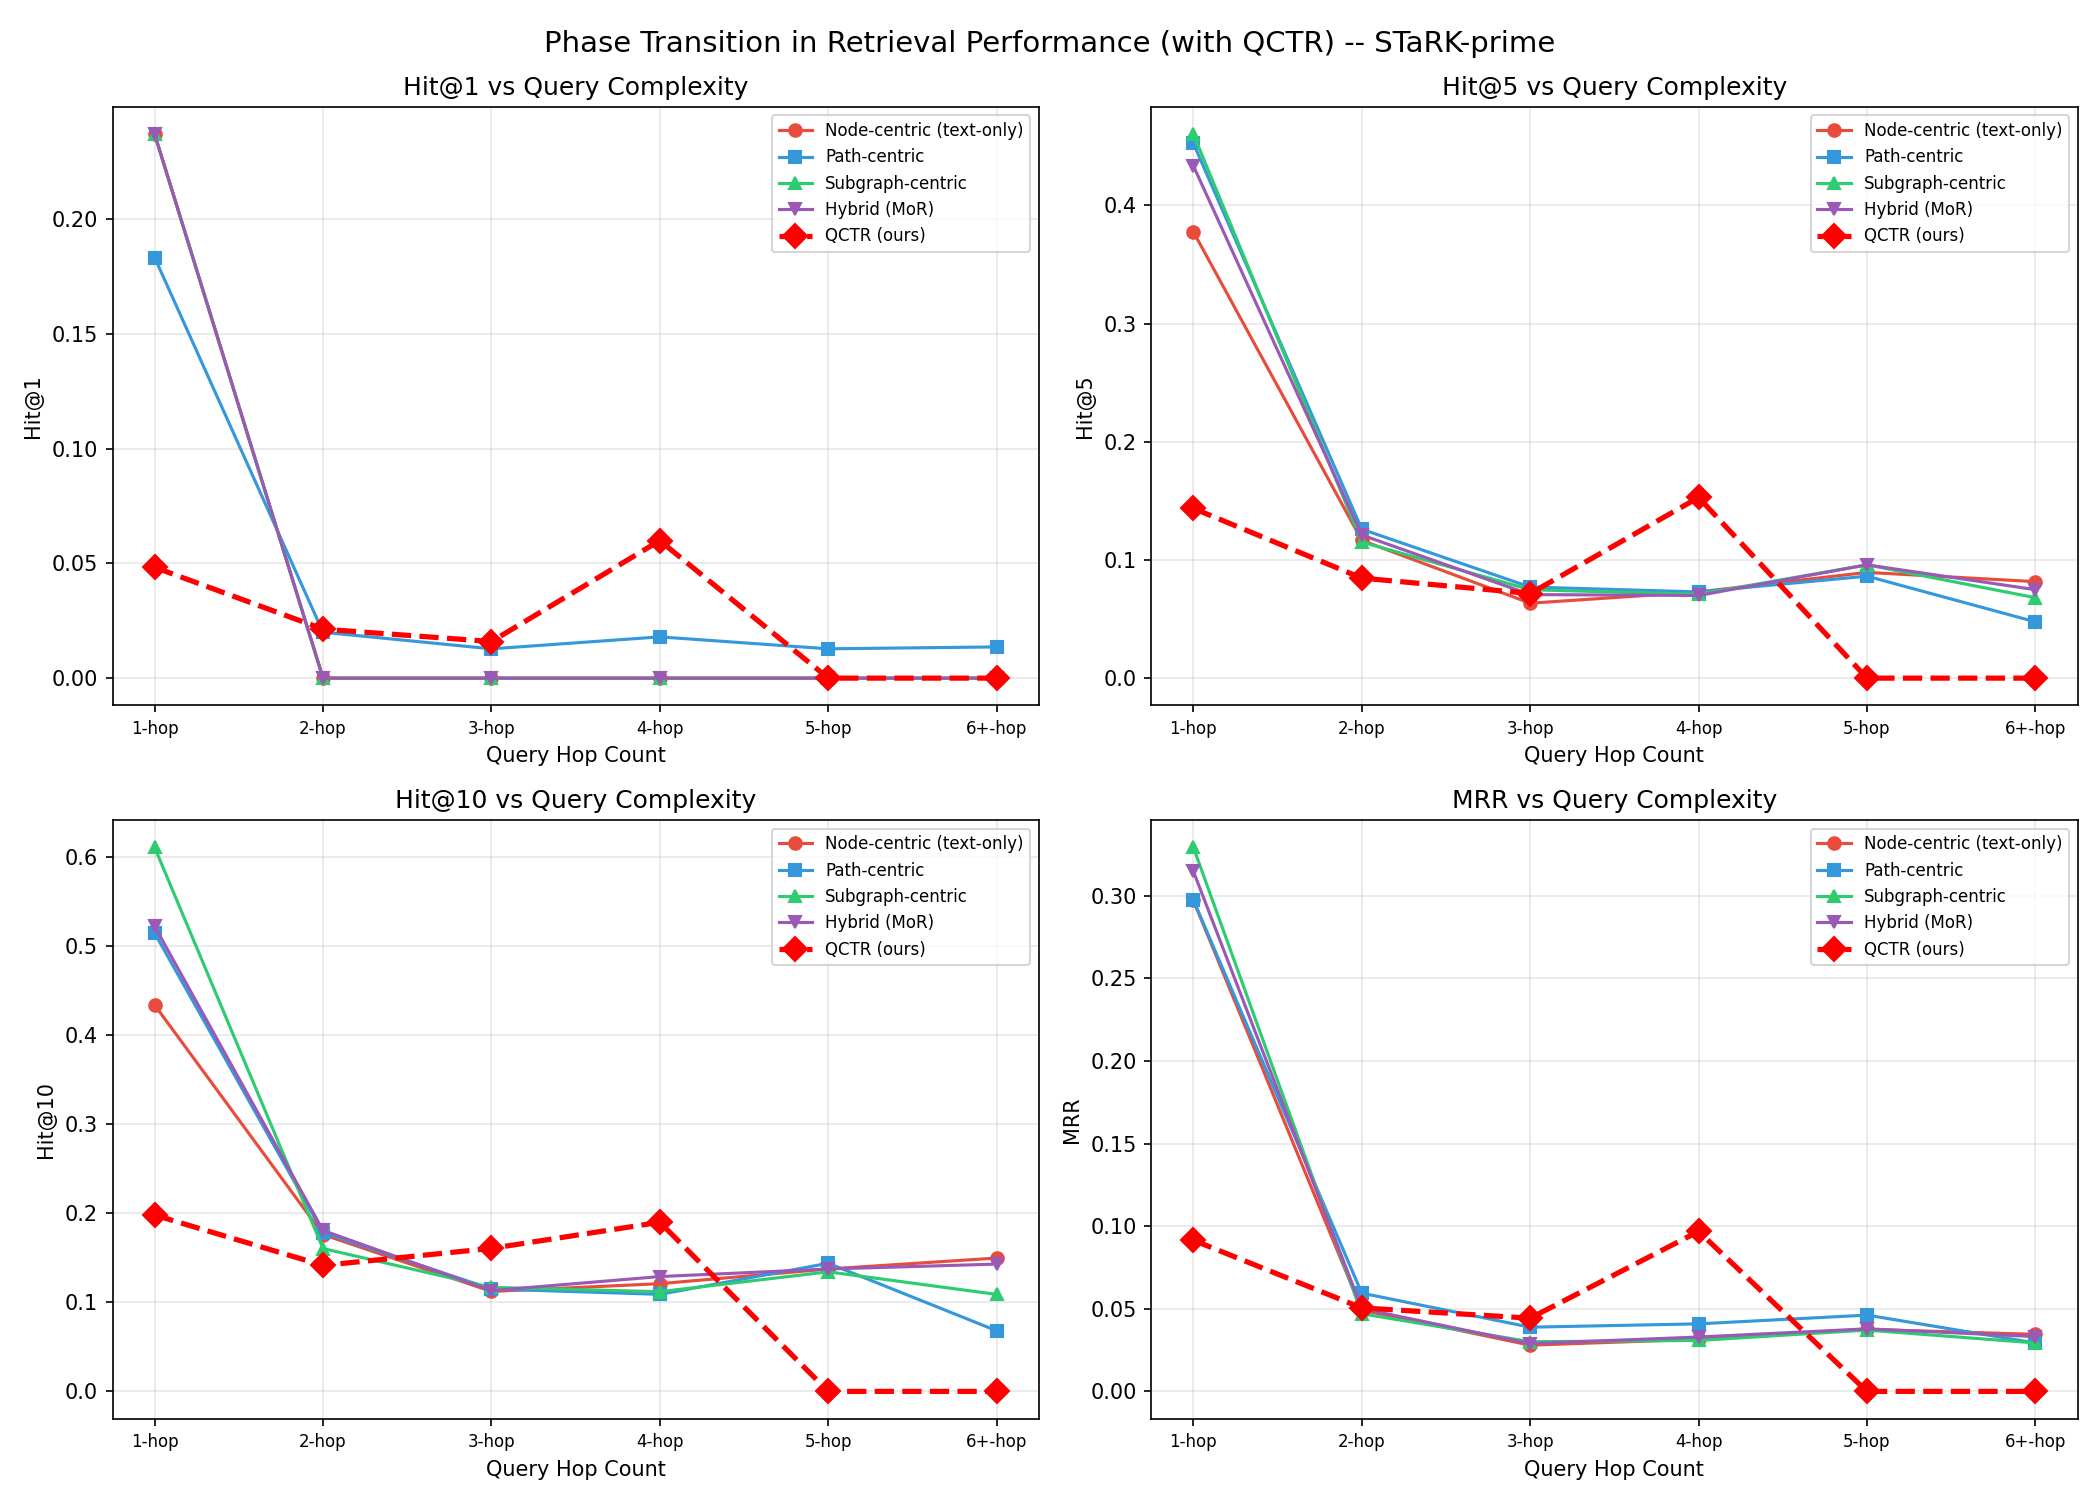
\includegraphics[width=\textwidth]{../results/prime_phase_transition_qctr.png}
    \caption{Phase transition plot with QCTR (red dashed). QCTR breaks above the baseline plateau at 3--4 hops but cannot reach 5+ hop answers. The 1$\to$2 hop cliff persists.}
    \label{fig:qctr_phase}
\end{figure}

\paragraph{Ablation study.} Table~\ref{tab:qctr_ablations} presents ablations on 100 queries per hop bin isolating the contribution of each QCTR component.

\begin{table}[h]
\centering
\caption{QCTR ablation study (Hit@10, 100 queries/bin). Key finding: max\_hops=2 is best for 1--2 hop; learned scoring beats cosine at 4-hop; smaller beams outperform larger ones.}
\label{tab:qctr_ablations}
\begin{tabular}{l cccccc}
\toprule
Config & 1-hop & 2-hop & 3-hop & 4-hop & 5-hop & 6+-hop \\
\midrule
QCTR (full) & 0.180 & 0.080 & 0.120 & \textbf{0.150} & 0.000 & 0.000 \\
cosine-only beam & 0.060 & 0.120 & 0.160 & 0.130 & 0.000 & 0.000 \\
no edge types & \textbf{0.690} & 0.080 & 0.000 & 0.000 & 0.000 & 0.000 \\
beam\_width=5 & 0.280 & \textbf{0.140} & \textbf{0.140} & 0.140 & 0.000 & 0.000 \\
beam\_width=20 & 0.160 & 0.080 & 0.080 & 0.140 & 0.000 & 0.000 \\
max\_hops=2 & 0.580 & \textbf{0.260} & 0.000 & 0.000 & 0.000 & 0.000 \\
max\_hops=6 & 0.100 & 0.090 & 0.060 & 0.070 & \textbf{0.030} & \textbf{0.020} \\
\bottomrule
\end{tabular}
\end{table}

Three findings emerge: (1)~\textit{Smaller beams outperform larger ones} at 2--3 hops (beam\_width=5 achieves 0.140 vs.\ 0.080 for beam\_width=20), mirroring the focus-vs-coverage tradeoff. (2)~\textit{Shallow search dominates for nearby answers}: max\_hops=2 achieves the best 2-hop Hit@10 (0.260) by concentrating search, but zeros out at 3+ hops. (3)~\textit{Edge types help at depth but hurt at surface}: removing edge embeddings yields 0.690 Hit@10 at 1-hop (best in any experiment) but collapses at 3+ hops, showing that relation-type constraints channel search toward multi-hop paths at the cost of flexibility for direct retrieval.

\paragraph{Bridge entity recall.} The key mechanistic question is whether QCTR actually preserves bridge entities---the intermediate nodes that embedding similarity discards. On 100 two-hop queries, we measure whether the correct bridge node (the intermediate node on the gold shortest path) appears in the beam after the first hop:

\begin{center}
\begin{tabular}{lc}
\toprule
Scorer & Bridge entity recall \\
\midrule
Learned (QCTR) & \textbf{75.0\%} (75/100) \\
Cosine & 55.0\% (55/100) \\
\bottomrule
\end{tabular}
\end{center}

QCTR retains 20 percentage points more bridge entities, confirming that the learned scorer identifies structurally important nodes that lack textual similarity to the query. This is the core mechanism by which QCTR improves multi-hop retrieval.

\paragraph{Density sensitivity.} We partition queries by the degree of their query entity (above/below median) and evaluate QCTR:

\begin{center}
\begin{tabular}{lcc}
\toprule
Hop & Low degree Hit@10 & High degree Hit@10 \\
\midrule
2-hop & \textbf{0.140} & 0.020 \\
3-hop & \textbf{0.160} & 0.080 \\
\bottomrule
\end{tabular}
\end{center}

QCTR performs 7$\times$ better on low-degree query nodes at 2-hop, providing direct evidence that density is the governing variable even \textit{within} a single graph. High-degree neighborhoods overwhelm the learned scorer just as they overwhelm cosine similarity, though with a higher threshold.

\paragraph{Decomposing the cliff.} QCTR reveals that the hop-count cliff comprises two distinct mechanisms:
\begin{enumerate}
    \item \textbf{Bridge entity pruning} (addressable): Embedding similarity discards intermediate nodes needed for multi-hop paths. QCTR's learned scorer partially solves this, improving 3--4 hop retrieval by 2--3$\times$.
    \item \textbf{Combinatorial explosion} (intrinsic): On dense graphs, the candidate set grows as $\bar{d}^h$, eventually overwhelming \textit{any} bounded-depth scorer. This explains why QCTR does not shift the 1$\to$2 hop cliff boundary and collapses at 5+ hops.
\end{enumerate}

\subsection{Cross-Domain Replication: The Role of Graph Density}

To test whether the cliff is specific to PrimeKG or a general phenomenon, we replicate on STaRK-Amazon, a much sparser graph (mean degree 9.1 vs.\ 62.6). Figure~\ref{fig:cross_domain} compares performance degradation across the two datasets.

\begin{figure}[h]
    \centering
    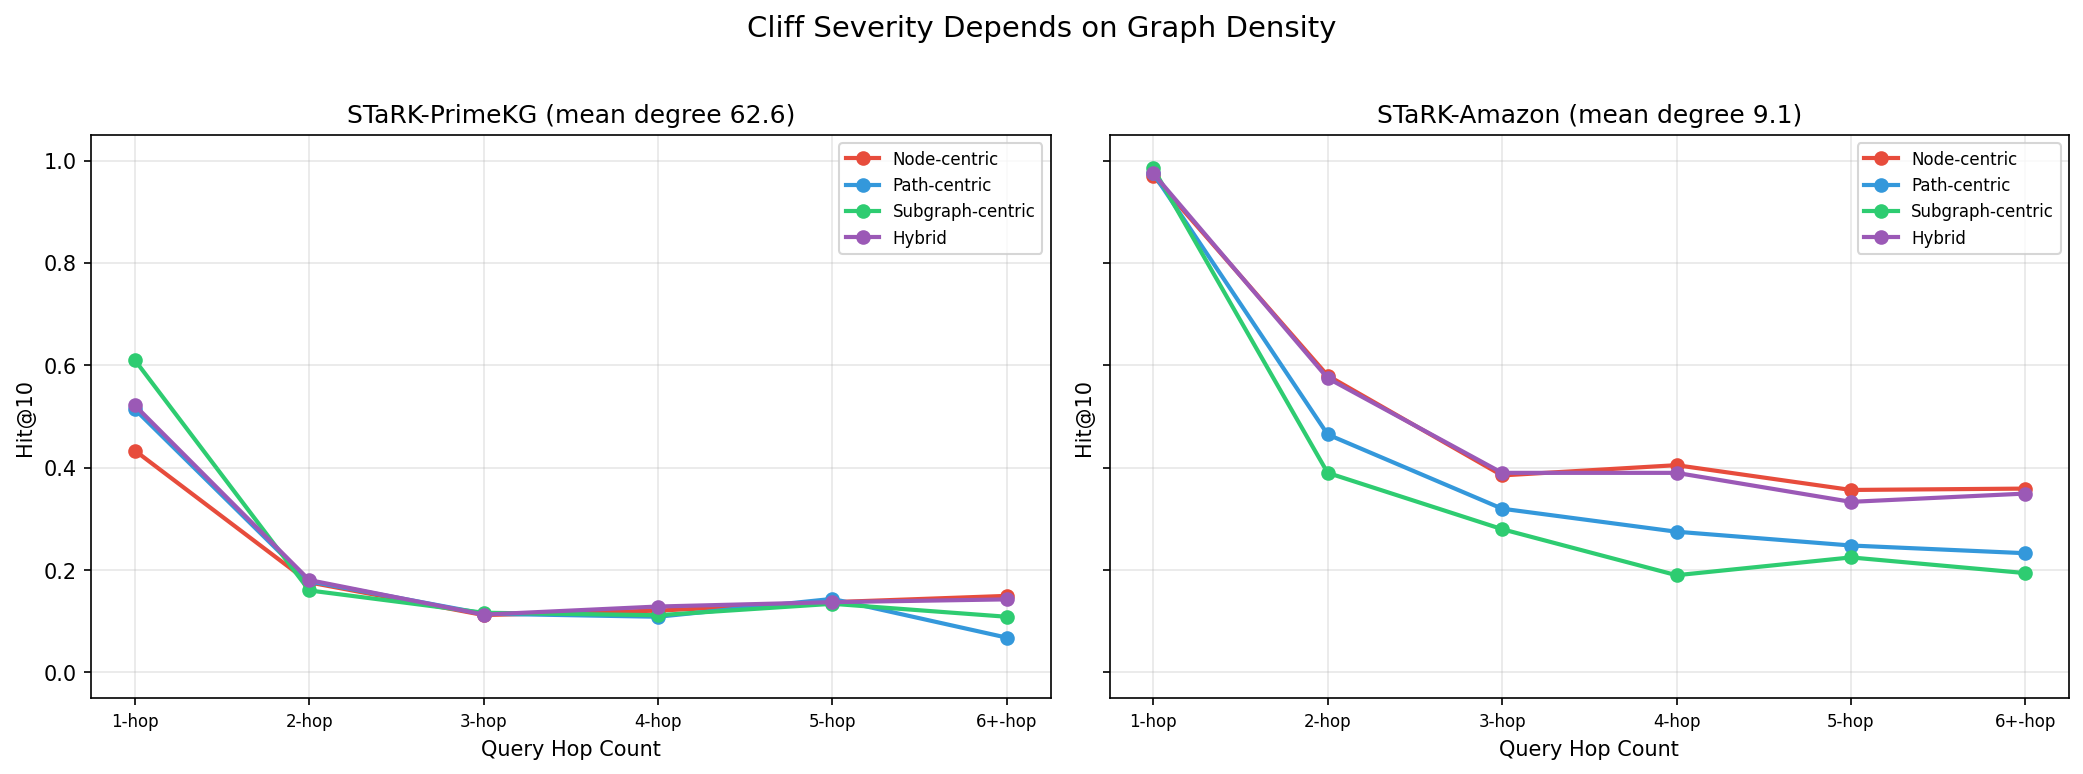
\includegraphics[width=\textwidth]{../results/cross_domain_hit10.png}
    \caption{Hit@10 vs.\ hop count on PrimeKG (dense, left) and Amazon (sparse, right). The cliff is severe on dense PrimeKG but gradual on sparse Amazon.}
    \label{fig:cross_domain}
\end{figure}

Table~\ref{tab:amazon_results} shows the Amazon results. Three striking differences emerge:

\begin{table}[h]
\centering
\caption{Hit@10 by hop count and strategy on STaRK-Amazon ($n = 200$/bin). Bold indicates best per row.}
\label{tab:amazon_results}
\begin{tabular}{l cccc}
\toprule
Hop & Node & Path & Subgraph & Hybrid \\
\midrule
1 & 0.970 & 0.975 & \textbf{0.985} & 0.975 \\
2 & \textbf{0.580} & 0.465 & 0.390 & 0.575 \\
3 & 0.385 & 0.320 & 0.280 & \textbf{0.390} \\
4 & \textbf{0.405} & 0.275 & 0.190 & 0.390 \\
5 & \textbf{0.357} & 0.248 & 0.225 & 0.333 \\
6+ & \textbf{0.359} & 0.233 & 0.194 & 0.350 \\
\bottomrule
\end{tabular}
\end{table}

\begin{enumerate}
    \item \textbf{The cliff is softer.} Hit@10 drops from 0.98 to 0.58 at 2-hop ($\sim$40\% drop) compared to PrimeKG's 70\% drop. Performance degrades gradually rather than catastrophically (Figure~\ref{fig:normalized}).
    \item \textbf{Node-centric beats structural methods at multi-hop.} On dense PrimeKG, subgraph-centric excels at 1-hop. On sparse Amazon, \textit{node-centric outperforms all structural methods} at 2+ hops. Structural expansion on a sparse graph adds too few neighbors ($\sim$9 per hop) to provide meaningful coverage, while potentially introducing noise.
    \item \textbf{Subgraph-centric is worst at multi-hop}---the opposite of its PrimeKG behavior. This confirms that the value of structural retrieval depends critically on graph density.
\end{enumerate}

\begin{figure}[h]
    \centering
    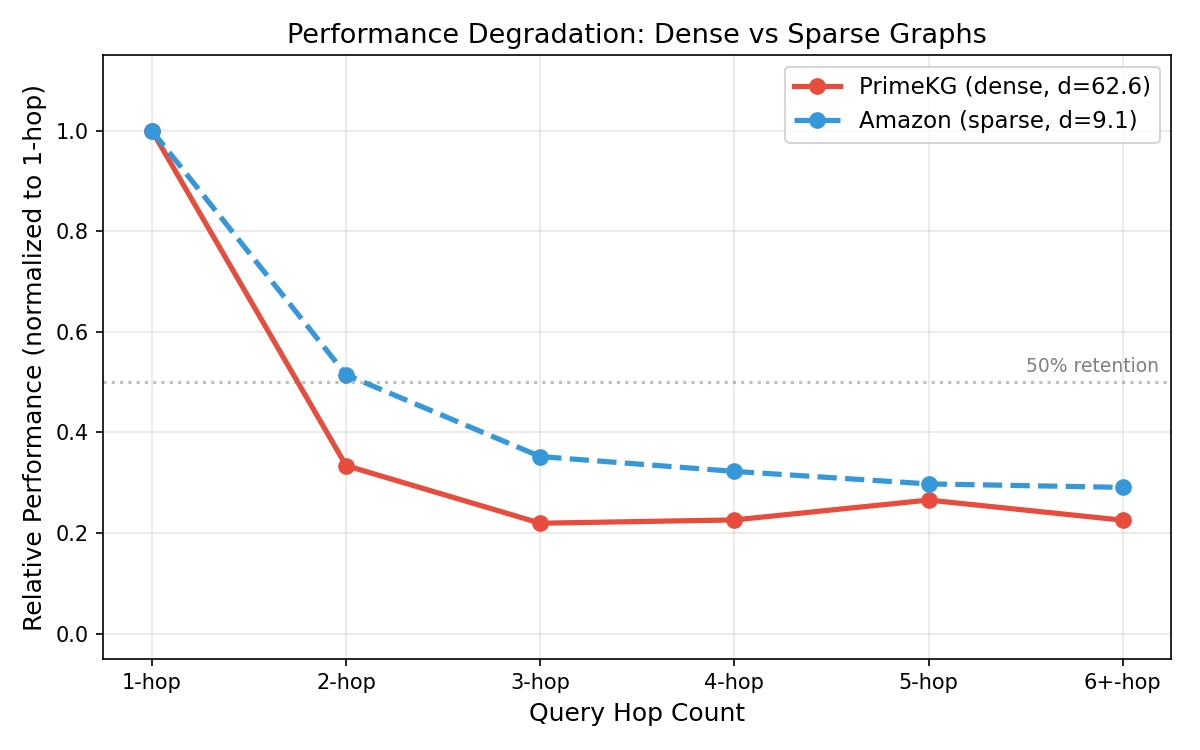
\includegraphics[width=0.7\textwidth]{../results/cross_domain_normalized.png}
    \caption{Performance retention relative to 1-hop (averaged across strategies). Dense PrimeKG loses 70\% of performance at 2-hop; sparse Amazon retains 60\%.}
    \label{fig:normalized}
\end{figure}

%----------------------------------------------------------------------
\section{Discussion}
%----------------------------------------------------------------------

\subsection{Why the Cliff?}

The hop-count cliff is a consequence of graph density. On STaRK-PrimeKG, the mean degree is 62.6, meaning a single hop from a query entity reaches $\sim$60 nodes. At 1-hop, the answer is likely within this immediate neighborhood, and all structural methods can find it. At 2-hop, the answer is somewhere among $\sim$3,600 second-degree neighbors, and embedding similarity alone cannot reliably distinguish the correct answer from thousands of structurally similar alternatives.

The Amazon replication confirms this explanation: with mean degree 9.1, a 2-hop expansion touches only $\sim$80 nodes, and the cliff is correspondingly softer. The relationship between density and cliff severity is consistent with a combinatorial argument: the number of candidate nodes at hop $h$ scales as $\bar{d}^h$, and embedding-based ranking fails when this number exceeds the effective discriminative capacity of the embedding space.

This also explains why structural methods hurt on sparse Amazon: when the neighborhood is small, expanding it adds little information but can introduce noise. The benefit of structure requires a ``Goldilocks zone'' of density where expansion reaches the answer but doesn't overwhelm the ranker.

\subsection{The Focus-vs-Coverage Tradeoff}

Our ablations reveal that every hyperparameter controlling retrieval breadth (number of seeds, expansion depth, path length, text weight) exhibits the same pattern: settings that maximize 1-hop performance minimize multi-hop performance and vice versa. This is not a limitation of our specific implementations but a structural property of retrieval on dense graphs: \textit{the information needed to reach multi-hop answers is diffused across many graph paths, and any strategy that focuses enough to avoid noise at 1-hop will miss the signal at higher hops.}

\subsection{Connections to Prior Work}

Our results provide empirical grounding for observations in the literature:
\begin{itemize}
    \item \citet{yue2025mor}'s ``uneven performance across query logics'' is not merely uneven---it is a cliff, with fundamentally different regimes above and below 2 hops.
    \item \citet{yu2025graphflow}'s finding that GraphRAG ``doesn't always retrieve what you need'' is explained by the density-driven noise that overwhelms structural signal at higher hop counts.
    \item The success of \citet{yue2025mor}'s planning stage can be understood as an implicit mechanism for adapting retrieval breadth to estimated query complexity.
\end{itemize}

\subsection{Implications}

Our results suggest that effective GraphRAG on dense knowledge graphs requires moving beyond pure embedding similarity. The cliff has two components, each suggesting a different remedy:

\begin{enumerate}
    \item \textbf{Bridge entity pruning} $\to$ \textbf{learned transition scoring}: QCTR demonstrates that training a scorer on shortest-path trajectories can recover bridge entities that cosine similarity discards. This is a lightweight intervention (an MLP with 732K parameters, no LLM calls) that significantly improves 3--4 hop retrieval. However, the gains are bounded by beam depth and do not address the combinatorial explosion.
    \item \textbf{Combinatorial explosion} $\to$ \textbf{relation-type-aware traversal or iterative retrieval}: On typed KGs like PrimeKG, filtering edges by relation type could reduce the effective degree from $\sim$60 to $\sim$10 per hop. QCTR's edge-type ablation supports this: removing edge types yields excellent 1-hop retrieval but collapses at multi-hop, showing that relation types are essential for channeling deep search. Alternatively, iterative retrieval-generation~\citep{trivedi2023ircot} decomposes multi-hop problems into sequential single-hop retrievals, avoiding the neighborhood explosion entirely.
\end{enumerate}

The most promising direction may be combining QCTR's learned transition scoring with relation-type filtering and iterative LLM-guided decomposition, attacking both failure mechanisms simultaneously.

\subsection{Limitations}

Our retrievers are relatively simple implementations that serve as controlled baselines rather than state-of-the-art systems. The papers we build on use more sophisticated approaches (learned planners, GNN encoders, LLM-guided traversal). Our contribution is characterizing the hop-count cliff and the density dependence, not claiming that our implementations are optimal.

While we evaluate on two domains (biomedical and e-commerce) spanning a wide range of graph densities, our density comparison is between two points. A more thorough investigation would sweep density continuously, e.g., by subsampling edges from a dense graph.

Our hop-count stratification relies on identifying the query entity via embedding similarity, which introduces noise. Some queries may be assigned to incorrect hop-count bins, potentially smoothing the observed cliff. The true cliff may be even sharper than we report.

%----------------------------------------------------------------------
\section{Conclusion}
%----------------------------------------------------------------------

We set out to find a phase transition in GraphRAG retrieval performance and found something more nuanced: a \textit{density-dependent cliff}. On dense knowledge graphs (PrimeKG, $\bar{d} = 62.6$), all retrieval strategies collapse at 2-hop queries with a $\sim$70\% performance drop. On sparse graphs (Amazon, $\bar{d} = 9.1$), the degradation is gradual ($\sim$40\%), and structural methods can even \textit{hurt}---the opposite of dense-graph behavior.

Through systematic ablation studies, we show that the cliff arises from a fundamental focus-versus-coverage tradeoff driven by the combinatorial explosion of neighborhoods on dense graphs. Beam search and adaptive routing experiments show the cliff is robust to principled attempts to overcome it within the embedding-based paradigm. Our QCTR method---which replaces embedding similarity with a learned query-conditioned transition scorer---partially breaks through the cliff, achieving 2--3$\times$ improvements at 3--4 hops ($p < 0.001$) and 75\% bridge entity recall vs.\ 55\% for cosine scoring. However, QCTR does not shift the 1$\to$2 hop cliff boundary, revealing that the cliff comprises two distinct mechanisms: an addressable \textit{pruning failure} at bridge entities, and an intrinsic \textit{combinatorial barrier} that overwhelms any bounded-depth scorer on dense graphs.

The cross-domain comparison reveals graph density as the key moderating variable for GraphRAG system design. On sparse graphs, simple text-based retrieval suffices even for multi-hop queries. On dense graphs, overcoming the cliff requires attacking both failure mechanisms: learned transition scoring (as in QCTR) to preserve bridge entities, combined with relation-type filtering or iterative retrieval-generation to manage the combinatorial explosion.

%----------------------------------------------------------------------
\bibliographystyle{plainnat}
\begin{thebibliography}{10}

\bibitem[Chandak et al.(2023)]{chandak2023primekg}
Chandak, P., Huang, K., and Zitnik, M.
\newblock Building a knowledge graph to enable precision medicine.
\newblock \textit{Scientific Data}, 10(67), 2023.

\bibitem[Hu et al.(2024)]{hu2024grag}
Hu, Y., Lei, Z., Zhang, Z., Pan, B., Ling, C., and Zhao, L.
\newblock GRAG: Graph Retrieval-Augmented Generation.
\newblock \textit{arXiv preprint arXiv:2405.16506}, 2024.

\bibitem[Lewis et al.(2020)]{lewis2020retrieval}
Lewis, P., Perez, E., Piktus, A., Petroni, F., Karpukhin, V., Goyal, N., K{\"u}ttler, H., Lewis, M., Yih, W., Rockt{\"a}schel, T., et~al.
\newblock Retrieval-augmented generation for knowledge-intensive NLP tasks.
\newblock \textit{NeurIPS}, 2020.

\bibitem[Sun et al.(2024)]{sun2024tog}
Sun, J., Xu, C., Tang, L., Wang, S., Lin, C., Gong, Y., Shum, H., and Guo, J.
\newblock Think-on-Graph: Deep and responsible reasoning of large language model on knowledge graph.
\newblock \textit{ICLR}, 2024.

\bibitem[Trivedi et al.(2023)]{trivedi2023ircot}
Trivedi, H., Balasubramanian, N., Khot, T., and Sabharwal, A.
\newblock Interleaving retrieval with chain-of-thought reasoning for knowledge-intensive multi-step questions.
\newblock \textit{ACL}, 2023.

\bibitem[Wang et al.(2025)]{wang2025skewroute}
Wang, H., et~al.
\newblock SkewRoute: Training-free LLM routing for KG-RAG via score skewness of retrieved context.
\newblock \textit{Findings of EMNLP}, 2025.

\bibitem[Alon and Yahav(2021)]{alon2021}
Alon, U. and Yahav, E.
\newblock On the bottleneck of graph neural networks and its practical implications.
\newblock \textit{ICLR}, 2021.

\bibitem[Di~Giovanni et al.(2023)]{digiovanni2023}
Di~Giovanni, F., Giusti, L., Barbero, F., Luise, G., Li\`{o}, P., and Bronstein, M.
\newblock On over-squashing in message passing neural networks: The impact of width, depth, and topology.
\newblock \textit{ICML}, 2023.

\bibitem[Green and Swets(1966)]{green1966}
Green, D. and Swets, J.
\newblock \textit{Signal Detection Theory and Psychophysics}.
\newblock Wiley, 1966.

\bibitem[Hoory et al.(2006)]{hoory2006}
Hoory, S., Linial, N., and Wigderson, A.
\newblock Expander graphs and their applications.
\newblock \textit{Bulletin of the AMS}, 43(4):439--561, 2006.

\bibitem[Johnson and Lindenstrauss(1984)]{johnson1984}
Johnson, W. and Lindenstrauss, J.
\newblock Extensions of Lipschitz mappings into a Hilbert space.
\newblock \textit{Contemporary Mathematics}, 26:189--206, 1984.

\bibitem[Reimers and Gurevych(2019)]{reimers2019sentence}
Reimers, N. and Gurevych, I.
\newblock Sentence-BERT: Sentence embeddings using Siamese BERT-networks.
\newblock \textit{EMNLP}, 2019.

\bibitem[Spielman(2025)]{spielman2025}
Spielman, D.
\newblock Spectral and Algebraic Graph Theory.
\newblock Yale University, 2025 draft.

\bibitem[Topping et al.(2022)]{topping2022}
Topping, J., Di~Giovanni, F., Chamberlain, B., Dong, X., and Bronstein, M.
\newblock Understanding over-squashing and bottlenecks on graphs via curvature.
\newblock \textit{ICLR}, 2022.

\bibitem[van~der~Hofstad(2017)]{vanderhofstad2017}
van~der~Hofstad, R.
\newblock \textit{Random Graphs and Complex Networks, Vol.\ I}.
\newblock Cambridge University Press, 2017.

\bibitem[Weller et al.(2025)]{weller2025}
Weller, O., Marone, M., Braverman, V., Dawn, J., and Van~Durme, B.
\newblock On the theoretical limitations of embedding-based retrieval.
\newblock \textit{arXiv preprint arXiv:2508.21038}, 2025.

\bibitem[Wu et al.(2024)]{wu2024stark}
Wu, S., et~al.
\newblock STaRK: Benchmarking LLM retrieval on textual and relational knowledge bases.
\newblock \textit{NeurIPS Datasets and Benchmarks}, 2024.

\bibitem[Yu et al.(2025)]{yu2025graphflow}
Yu, J., Liu, Y., Gu, J., Torr, P., and Zhou, D.
\newblock Can knowledge-graph-based retrieval augmented generation really retrieve what you need?
\newblock \textit{NeurIPS}, 2025.

\bibitem[Yue et al.(2025)]{yue2025mor}
Yue, Z., et~al.
\newblock Mixture of structural-and-textual retrieval over text-rich graph knowledge bases.
\newblock \textit{Findings of ACL}, 2025.

\end{thebibliography}

\end{document}
